\documentclass{article}
\usepackage{graphicx} % Required for inserting images
\usepackage{amsmath}
\usepackage{hyperref}

\title{Asssignment 4}
\author{Atharva}
\date{June 2023}

\begin{document}

\maketitle

\section*{MM22B006}
Name: Atharva Kulkarni\\
Github user-id: Error404Occured

\subsection*{History of Pythagoras theorem}

Pythagoras' theorem was proposed by the Pythagoras of Samos, a Greek mathematician. He was an ancient Greek philosopher who founded a group of mathematicians who lived as monks and worked passionately on numbers. Although Pythagoras popularised the theorem, there is evidence that it existed in other civilizations 1000 years before Pythagoras. The earliest known proof is from the 20th to the 16th centuries B.C. in the Old Babylonian Period.

\subsection*{Pythagoras Theorem Statement}\footnote{Reference:\url{https://byjus.com/maths/pythagoras-theorem/}}

Pythagoras theorem states, "In a right-angled triangle, the square of the hypotenuse side is equal to the sum of squares of the other two sides".

\subsection*{Pythagoras Theorem Formula}


Consider the triangle given above:
Where “a” is the perpendicular,
“b” is the base,
“c” is the hypotenuse.
According to the definition, the Pythagoras Theorem formula is given as:

\begin{equation}
    a^2 + b^2 \boldsymbol{=} c^2
\end{equation}

\begin{figure}[h!t]
    \centering
    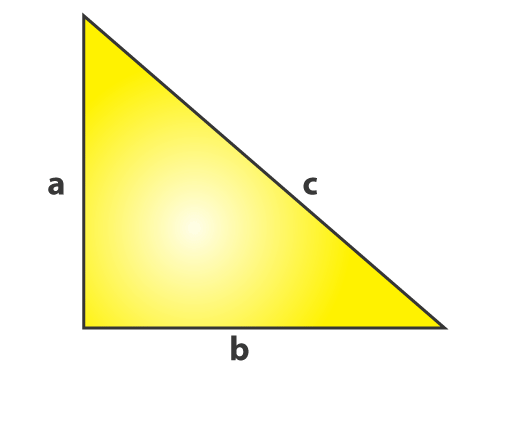
\includegraphics[width=0.5\textwidth]{P1.png}
    \caption{Right Angled Triangle}
    \label{fig:my_label1}
\end{figure}


\subsection*{Pythagoras Theorem Proof}

Given: A right-angled triangle ABC, right-angled at B.


To Prove-
\begin{equation}
    AC^2 \boldsymbol{=} AB^2 + BC^2
\end{equation}

Construction: Draw a perpendicular BD meeting AC at D

\begin{figure}
    \centering
    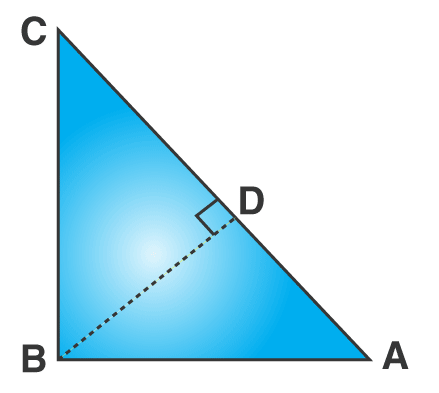
\includegraphics[width=0.5\textwidth]{P2.png}
    \caption{Pythagoras Theorem Proof}
    \label{fig:my_label2}
\end{figure}

We know, $\triangle ABD \sim \triangle ABC$. Therefore,
\[
\frac{AB}{AD} \boldsymbol{=} \frac{AC}{AB} \quad \text{(corresponding side of similiar triangles)}
\]

Or,
$AB^2 \boldsymbol{=} AD \times AC \quad \dots \quad (1)$ 

Also, $\triangle BDC \sim \triangle ABC$. Therefore,
\[
AB^2 + BC^2 \boldsymbol{=} AD \times AC + CD \times AC
\]

\[
AB^2 +BC^2 \boldsymbol{=} AC (AC + CD)
\]

Since $AD +CD \boldsymbol{=} AC$, we have

\[
AC^2 \boldsymbol{=} AB^2 + BC^2
\]

Hence, the Pythagorean theorem is proved.

\subsection*{Applications}\footnote{Source:\url{https://www.cuemath.com/geometry/pythagoras-theorem/}}

\begin{itemize}
        \item To know if the triangle is a right-angled triangle or not.
        \item In a right-angled triangle, we can calculate the length of any side if the other two sides are given.
        \item To find the diagonal of a square.
\end{itemize}


\subsection*{Use of Pythagorus Theorem}

\begin{itemize}
        \item Engineering and Construction fields
        \item Face recognition in security cameras
        \item Woodwork and interior designing
        \item Navigation
\end{itemize}

\end{document}
